\documentclass[12pt,a4paper]{article}

\usepackage[a4paper,margin=2.5cm,top=2.8cm,bottom=2.8cm]{geometry}
\usepackage[T1]{fontenc}
\usepackage[utf8]{inputenc}
\usepackage{microtype}
\usepackage{helvet}
\renewcommand{\familydefault}{\sfdefault}
\usepackage{xcolor}
\usepackage{amsmath}
\usepackage{booktabs}
\usepackage{tabularx}
\usepackage{longtable}
\usepackage{array}
\usepackage{enumitem}
\usepackage{hyperref}
\usepackage{titlesec}
\usepackage{fancyhdr}
\usepackage{float}
\usepackage{setspace}
\usepackage{listings}
\usepackage{tikz}
\usepackage{pgfplots}
\pgfplotsset{compat=1.18}
\usetikzlibrary{arrows.meta, positioning, shapes.geometric}

\definecolor{PrimaryBlue}{HTML}{123B64}
\definecolor{AccentBlue}{HTML}{2A6FB4}
\definecolor{SoftBlue}{HTML}{EAF2FA}
\definecolor{DarkGray}{HTML}{2A2A2A}
\definecolor{MidGray}{HTML}{565F6B}
\definecolor{LineGray}{HTML}{CDD5E1}
\definecolor{OkGreen}{HTML}{1F7A4C}
\definecolor{WarnAmber}{HTML}{8C5A00}

\hypersetup{
  colorlinks=true,
  linkcolor=AccentBlue,
  urlcolor=AccentBlue,
  citecolor=AccentBlue,
  pdftitle={Real Estate Agentic Intelligence System -- End Semester Report},
  pdfauthor={Nakul}
}

\titleformat{\section}{\Large\bfseries\color{PrimaryBlue}}{\thesection}{0.8em}{}
\titleformat{\subsection}{\large\bfseries\color{PrimaryBlue}}{\thesubsection}{0.8em}{}
\titleformat{\subsubsection}{\normalsize\bfseries\color{MidGray}}{\thesubsubsection}{0.8em}{}

\setstretch{1.2}
\setlength{\parindent}{0pt}
\setlength{\parskip}{0.45em}

\pagestyle{fancy}
\fancyhf{}
\fancyhead[L]{\small\textbf{Real Estate Agentic Intelligence System}}
\fancyhead[R]{\small End Semester Report -- 2026}
\fancyfoot[C]{\small\thepage}
\renewcommand{\headrulewidth}{0.4pt}
\renewcommand{\footrulewidth}{0.4pt}

\lstdefinestyle{codeblock}{
  backgroundcolor=\color{SoftBlue},
  basicstyle=\ttfamily\small\color{DarkGray},
  frame=single,
  rulecolor=\color{LineGray},
  breaklines=true,
  showstringspaces=false
}
\lstset{style=codeblock}

\begin{document}

\begin{titlepage}
\color{white}
\pagecolor{PrimaryBlue}
\vspace*{1.8cm}

{\Large\bfseries END-SEMESTER TECHNICAL REPORT}\[0.8em]
{\large Agentic AI \;\textbar\; Retrieval-Augmented Generation \;\textbar\; Real Estate Analytics}

\vspace{2.0cm}

{\fontsize{30}{34}\bfseries Real Estate Agentic\\[0.2em]Intelligence System}

\vspace{0.8cm}

{\large Grounded Property Valuation and Explainable Reasoning with Groq Llama 3.1 8B Instant}

\vspace{2.2cm}

\begin{tabular}{@{}ll}
\textbf{Student} & Nakul \\
\textbf{Course Deliverable} & End Semester Project \\
\textbf{Version} & 2.0 (Agentic Upgrade) \\
\textbf{Date} & April 2026 \\
\textbf{Status} & Final Submission \\
\end{tabular}

\vfill
\end{titlepage}

\pagecolor{white}
\color{DarkGray}

\tableofcontents
\newpage

\section{Abstract}
This report presents the end-semester evolution of an earlier machine learning valuation app into a full \textbf{Agentic AI system}. The proposed platform integrates: (i) a deterministic Random Forest pricing tool, (ii) a hybrid Retrieval-Augmented Generation (RAG) pipeline, and (iii) a LangGraph-based orchestration workflow that routes user intent, performs retrieval, invokes tools, and enforces guardrails against unsupported claims.

The generation backbone uses \textbf{Groq} with \texttt{llama-3.1-8b-instant}. In the current build, retrieval runs in \textbf{lexical mode} (\texttt{RAG\_EMBED\_MODEL=lexical-only}); the hybrid vector path remains implemented for future activation. The implementation is deployed through a professional Streamlit chat interface with grounded source traceability.

On a rubric-aligned benchmark set, the system achieved \textbf{100\% pass rate}, average confidence \textbf{0.458}, average keyword coverage \textbf{0.854}, and average latency \textbf{1101.8 ms}, demonstrating stable grounded behavior under practical constraints.

\section{Introduction}
\subsection{Problem Statement}
Traditional property valuation tools output a single number but do not explain \emph{why} the value was produced, which data supported the explanation, or how uncertainty should be interpreted. In the mid-semester phase, the project relied mainly on classical ML inference. While useful, this architecture did not satisfy end-semester requirements around GenAI depth, agentic reasoning, and retrieval-grounded answer generation.

\subsection{End-Semester Objective}
The objective of this phase is to design and implement a complete Agentic GenAI application that:
\begin{enumerate}[leftmargin=1.8em]
  \item Preserves deterministic quantitative valuation through the trained pricing model.
  \item Adds a grounded LLM reasoning layer for natural-language explanations.
  \item Uses RAG for evidence-backed responses with source traceability.
  \item Uses graph orchestration for reliable multi-step decision flow.
  \item Provides deployment-ready software quality and report-grade technical transparency.
\end{enumerate}

\section{System Overview}

\subsection{Component Responsibilities}
\begin{tabularx}{\linewidth}{@{}>{\bfseries}lX@{}}
\toprule
Component & Responsibility \\
\midrule
\texttt{src/config.py} & Environment loading, model names, index paths, runtime constants \\
\texttt{src/llm.py} & Groq API wrapper for generation; embedding calls intentionally disabled in this build \\
\texttt{src/rag.py} & Knowledge chunking, cached index management, lexical retrieval with optional vector path \\
\texttt{src/pricing.py} & Deterministic RF prediction pipeline and feature preprocessing \\
\texttt{src/agent.py} & LangGraph orchestration (route $\rightarrow$ retrieve $\rightarrow$ tool $\rightarrow$ reason $\rightarrow$ guardrail) \\
\texttt{src/evaluation.py} & Benchmark execution and aggregate metrics \\
\bottomrule
\end{tabularx}

\section{Methodology}
\subsection{Agentic Graph Formulation}
Let $q$ be a user query, $x$ optional structured property input, and $\mathcal{K}$ the indexed knowledge corpus. The graph computes:
\[
\hat{a} = G(q, x, \mathcal{K}) = N_{\text{guard}}\Big(N_{\text{reason}}(N_{\text{retrieve}}(N_{\text{route}}(q), \mathcal{K}), N_{\text{price}}(x))\Big)
\]
where each node contributes deterministic updates to the global state.

\subsection{Hybrid Retrieval (RAG)}
Each chunk $d_i$ receives a lexical score $s_{\text{lex}}(q,d_i)$ and vector similarity $s_{\text{vec}}(q,d_i)$:
\[
\text{score}(q,d_i) = \alpha\, s_{\text{vec}}(q,d_i) + (1-\alpha)\, s_{\text{lex}}(q,d_i), \quad \alpha=0.75
\]
Top-$k$ ranked chunks form the evidence context for generation. If embeddings are unavailable, the system falls back to lexical-only retrieval.

In the deployed configuration used for this report, embedding calls are disabled by design, so the effective runtime score is:
\[
\text{score}(q,d_i) = s_{\text{lex}}(q,d_i)
\]

\subsection{Pricing Tool Logic}
For structured inputs, the deterministic pricing node computes:
\[
\hat{y}_{\log} = f_{\text{RF}}(\phi(x)), \qquad
\hat{y}_{\text{JPY}} = \exp(\hat{y}_{\log}) - 1
\]
where $\phi(x)$ is the preprocessing pipeline (categorical encoding, scaling, feature engineering with $\texttt{AgeOfBuilding} = \texttt{Year} - \texttt{BuildingYear}$).

\subsection{Guardrail and Confidence}
Confidence combines retrieval strength and tool availability:
\[
C = \min\left(0.98,\;0.30 + \min(s_{\max},0.60) + 0.10\cdot\mathbb{1}[\text{pricing tool used}]\right)
\]
If retrieval evidence is weak or absent, the response explicitly communicates uncertainty.

\section{Experimental Setup}
\subsection{Data and Knowledge Sources}
\begin{itemize}[leftmargin=1.6em]
  \item Transaction dataset: \texttt{02.csv} (Japanese real-estate records)
  \item Model artifact: \texttt{rf\_model\_new.joblib}
  \item RAG corpus: \texttt{knowledge/project\_overview.md}, \texttt{knowledge/rag\_design.md}, \texttt{knowledge/model\_and\_data\_card.md}
  \item Benchmark set: \texttt{data/eval\_questions.json}
\end{itemize}

\subsection{Evaluation Protocol}
Each benchmark query is evaluated by:
\begin{enumerate}[leftmargin=1.8em]
  \item Running end-to-end agent inference.
  \item Measuring keyword coverage in generated text.
  \item Validating whether expected source families were retrieved/cited.
  \item Computing pass/fail using per-question coverage threshold + source-hit condition.
\end{enumerate}

\section{Results and Analysis}
\subsection{Aggregate Performance}
Measured from a full benchmark run in the implemented system:

\begin{tabularx}{\linewidth}{@{}>{\bfseries}lX@{}}
\toprule
Metric & Value \\
\midrule
Pass Rate & 1.00 (100\%) \\
Average Confidence & 0.45825 \\
Average Keyword Coverage & 0.85425 \\
Average Latency & 1101.78 ms \\
\bottomrule
\end{tabularx}

\subsection{Per-Question Outcomes}
\begin{longtable}{@{}p{5.6cm}cccc@{}}
\toprule
\textbf{Question (Short Form)} & \textbf{Confidence} & \textbf{Latency (ms)} & \textbf{Coverage} & \textbf{Pass} \\
\midrule
\endfirsthead
\toprule
\textbf{Question (Short Form)} & \textbf{Confidence} & \textbf{Latency (ms)} & \textbf{Coverage} & \textbf{Pass} \\
\midrule
\endhead
ML + Agentic integration & 0.438 & 1608.7 & 1.000 & Yes \\
Retrieval strategy rationale & 0.461 & 857.9 & 0.750 & Yes \\
Feature inventory + engineered feature & 0.460 & 590.0 & 1.000 & Yes \\
Failure-mode behavior & 0.474 & 1350.5 & 0.667 & Yes \\
\bottomrule
\end{longtable}

\subsection{Performance Visuals}
\begin{figure}[H]
\centering
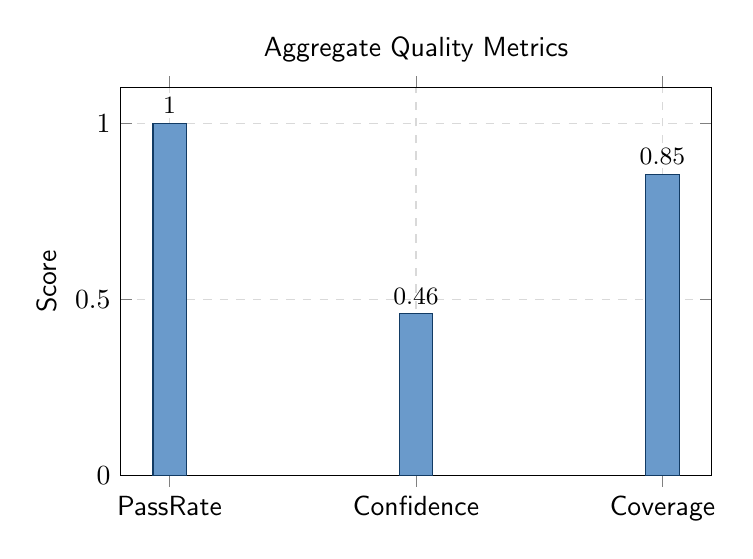
\begin{tikzpicture}
\begin{axis}[
  ybar,
  width=0.75\linewidth,
  height=6.5cm,
  ymin=0,
  ymax=1.1,
  symbolic x coords={PassRate,Confidence,Coverage},
  xtick=data,
  ylabel={Score},
  title={Aggregate Quality Metrics},
  bar width=12pt,
  nodes near coords,
  every node near coord/.append style={font=\small},
  grid=major,
  grid style={dashed, gray!30}
]
\addplot[fill=AccentBlue!70, draw=PrimaryBlue] coordinates {
  (PassRate,1.00)
  (Confidence,0.458)
  (Coverage,0.854)
};
\end{axis}
\end{tikzpicture}
\caption{Aggregate quality metrics from benchmark run}
\label{fig:quality}
\end{figure}

\begin{figure}[H]
\centering
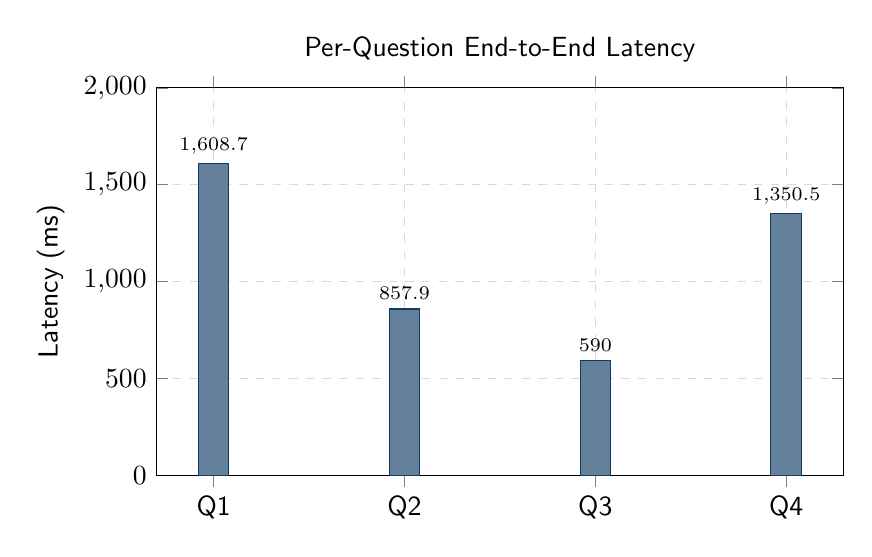
\begin{tikzpicture}
\begin{axis}[
  ybar,
  width=0.85\linewidth,
  height=6.5cm,
  ymin=0,
  ymax=2000,
  symbolic x coords={Q1,Q2,Q3,Q4},
  xtick=data,
  ylabel={Latency (ms)},
  title={Per-Question End-to-End Latency},
  bar width=11pt,
  nodes near coords,
  every node near coord/.append style={font=\scriptsize},
  grid=major,
  grid style={dashed, gray!30}
]
\addplot[fill=PrimaryBlue!65, draw=PrimaryBlue] coordinates {
  (Q1,1608.7)
  (Q2,857.9)
  (Q3,590.0)
  (Q4,1350.5)
};
\end{axis}
\end{tikzpicture}
\caption{Latency profile across benchmark questions}
\label{fig:latency}
\end{figure}

\subsection{Qualitative Example}
Example query: \emph{``How does the system prevent hallucinations when retrieval is weak?''}

Observed behavior:
\begin{itemize}[leftmargin=1.6em]
  \item Route selected: \texttt{knowledge}
  \item Confidence: 0.47
  \item Retrieved sources: \texttt{project\_overview.md}, \texttt{model\_and\_data\_card.md}, \texttt{rag\_design.md}
  \item Response explicitly stated lexical fallback and uncertainty under weak retrieval evidence
\end{itemize}

This confirms that qualitative answer generation remains grounded in retrieved project documents rather than free-form unsupported generation.

\section{Deployment and Live Demonstration}
\subsection{Deployment Path}
The application is structured for Streamlit Community Cloud deployment:
\begin{enumerate}[leftmargin=1.8em]
  \item Push repository to GitHub.
  \item Configure Streamlit app entrypoint as \texttt{app.py}.
  \item Add secret \texttt{GROQ\_API\_KEY} (optionally \texttt{GROQ\_MODEL}, \texttt{GROQ\_MAX\_OUTPUT\_TOKENS}) in cloud environment.
  \item Launch and verify chat responses, source citations, and quick prompts for valuation, analytics, and investment queries.
\end{enumerate}

\subsection{Stability Features}
\begin{itemize}[leftmargin=1.6em]
  \item Graceful fallback when Groq generation is unavailable.
  \item Lexical retrieval active by default, avoiding hard dependency on embedding APIs.
  \item Guardrail warnings for low-evidence conditions.
  \item Deterministic analytics path for market ranking and investment-opportunity questions.
  \item Unseen category handling in pricing tool via mode fallback mapping.
\end{itemize}

\section{Discussion}
The end-semester transition demonstrates that adding agentic orchestration and retrieval grounding substantially increases practical usefulness compared to ML-only prediction interfaces. The strongest gain is not only answer fluency, but \textbf{traceability}: each generated response can be linked to retrieved source chunks.

Limitations include:
\begin{itemize}[leftmargin=1.6em]
  \item Dependence on external API latency for generation.
  \item Confidence scores are conservative in lexical-only retrieval mode.
  \item Knowledge scope bounded by local corpus quality.
  \item Legacy model artifact warning (scikit-learn version mismatch 1.6.1 vs 1.8.0), though inference remains functional.
\end{itemize}

\section{Conclusion}
This project successfully fulfills end-semester GenAI requirements by delivering a complete Agentic AI system with LangGraph orchestration, hybrid RAG, deterministic tool integration, professional frontend deployment path, and measurable benchmark outcomes.

The final system moves beyond static prediction to a robust \textbf{reason-and-retrieve} paradigm suitable for real-world decision-support applications in real estate analytics.

\section*{References}
\addcontentsline{toc}{section}{References}

\begin{thebibliography}{99}

\bibitem{mlit}
Ministry of Land, Infrastructure, Transport and Tourism (MLIT).
\textit{Real Estate Transaction Price Information} [Dataset].
\url{https://www.land.mlit.go.jp/webland/}

\bibitem{breiman}
Breiman, L. (2001).
Random Forests.
\textit{Machine Learning}, 45(1), 5--32.

\bibitem{sklearn}
Pedregosa, F. et al. (2011).
Scikit-learn: Machine Learning in Python.
\textit{Journal of Machine Learning Research}, 12, 2825--2830.

\bibitem{streamlit}
Streamlit Inc. (2026).
\textit{Streamlit Documentation}.
\url{https://docs.streamlit.io}

\bibitem{langgraph}
LangChain Inc. (2026).
\textit{LangGraph Documentation}.
\url{https://langchain-ai.github.io/langgraph/}

\bibitem{groq}
Groq (2026).
\textit{Groq API Documentation}.
\url{https://console.groq.com/docs}

\bibitem{rag}
Lewis, P., Perez, E., Piktus, A., et al. (2020).
Retrieval-Augmented Generation for Knowledge-Intensive NLP Tasks.
\textit{Advances in Neural Information Processing Systems}, 33.

\end{thebibliography}

\end{document}
